\section{Backend}\label{sec:poc:backend}
\begin{figure}[ht]
  \centering
  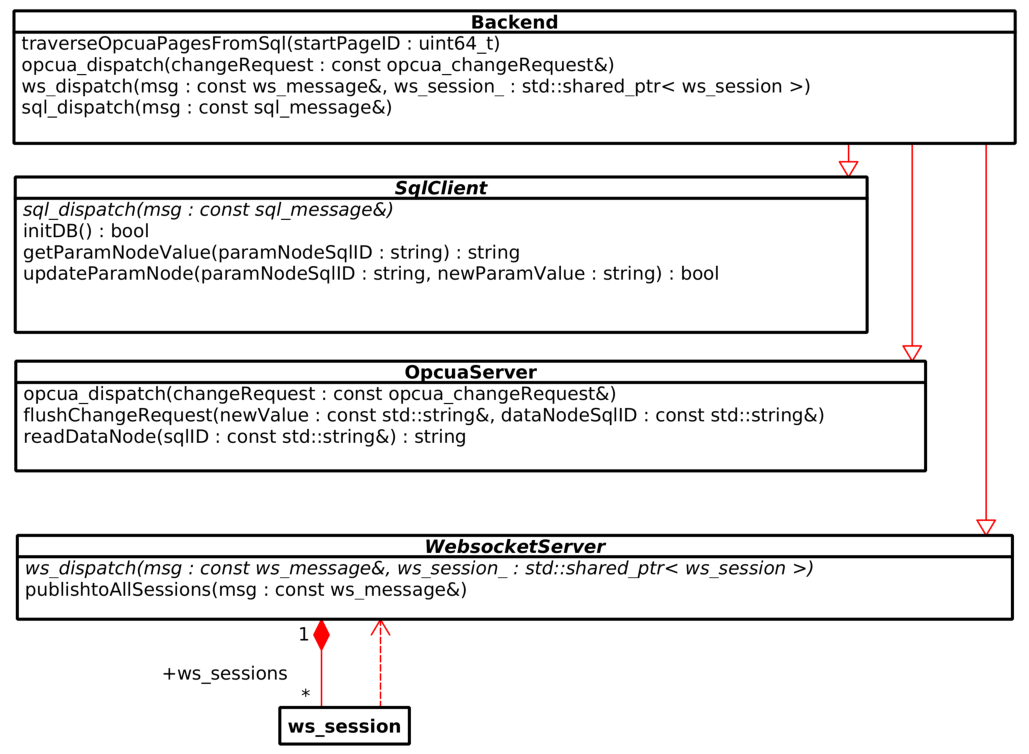
\includegraphics[width=\textwidth]{content/hauptteil/umsetzungPoC/backend/uml/overview.pdf}
  \caption{Klassendiagramm Überblick Backend}
  \label{fig:backend:classDiag:overview}
\end{figure}
Das Klassendiagramm in \refFig{fig:backend:classDiag:overview} stellt die Grundstruktur des Backends dar. 
Das Diagramm ist, bis auf die \eigenName{Backend} Klasse, nicht vollständig und auf die wesentlichen Operationen zur Kommunikation reduziert. 
Die \eigenName{Backend} Klasse (abgeleitete Klasse) erbt von den drei Basisklassen \eigenName{SqlClient}, \eigenName{OpcuaServer} und \eigenName{WebsocketServer}.
Jede Basisklasse hat ihre eigene dedizierte Aufgabe die in den einzelnen jeweiligen, gleichnamigen Abschnitten genauer beschrieben ist.
Die abgeleitete Klasse steht dabei als Vermittler dazwischen. Möchte eine der Basisklassen etwas ausführen, für das eine der anderen Klassen benötigt wird, 
so kann diese das anstoßen, indem sie eine virtuelle (genauer: \eigenName{pure virtual}) Methode aufruft, die in der Basisklasse selbst nicht implementiert wird, sondern in der abgeleiteten \eigenName{Backend} Klasse.
Dies ermöglicht es nun indirekt durch eine Basisklasse eine Methode einer anderen Basisklasse aufzurufen.
Um zu garantieren, dass dies auch geschieht und nicht durch einen Tippfehler eine falsche Methode aufgerufen wird, 
ist die Methode in der Basisklasse mit \eigenName{ = 0 } definiert, was den Versuch der Dereferenzierung dieser Methode verhindert und mit einem Kompilerfehler kennzeichnet.
Diese Eigenschaft einer Methode ist im Klassendiagramm durch die kursive Schrift der Operation gekennzeichnet.
In der abgeleiteten Klasse (\eigenName{Backend}) wird die dort reimplementierte Methode nun mit dem Schlüsselwort \eigenName{override} am Ende der Deklaration gekennzeichnet.
Dies zwingt den Kompiler zu überprüfen, ob die dort deklarierte Methode wirklich eine Methode der Basisklasse reimplementiert und nicht eine neue Methode ist.
Zusätzlich zu den virtuellen Methoden, die in diesem Fall eine Kommunikation zu anderen Basisklassen, indirekt über die abgeleitete Klasse, ermöglichen, existieren noch eine Anzahl an Methoden, 
über die man mit der Klasse selbst interagieren kann.
Die Methode \eigenName{traverseOpcuaPagesFromSql(startPageID)} erstellt alle notwendigen \ac{opcua} Nodes, auf Basis der Datenstruktur, ab der angegebenen \eigenName{startPageID}.

Eine Sonderrolle nehmen dabei die Operationen ein, die im Klassendiagramm von \refFig{fig:backend:classDiag:overview}, außer der bereits beschriebenen noch zusätzlich dargestellt sind.
Sie ermöglichen die Änderung oder Abfrage von Daten der jeweiligen Klassen.\\
%erwähnung datenaustausch zwischen basisklassen zu abgeleitetrer...(dispatcher.... )
  %endlich anzahl an fkt für daten backend -> basisklassen
  %pro basisklasse ein dispatcher im Backend (virtual) --> Verweis auf Kapitel
%erwähnung message klassen die geparsed wwerden ------- besser in einzelnen abschnitten
Die einzelnen Basisklassen sind zusätzlich separat in den Abbildungen 
\ref{fig:backend:classDiag:WebsocketServer}, \ref{fig:backend:classDiag:SqlClient} sowie \ref{fig:backend:classDiag:OpcuaServer} 
vollständig, mit allen Attributen und Operationen, dargestellt.
\subsection{WebsocketServer}
\begin{figure}[ht]
  \centering
  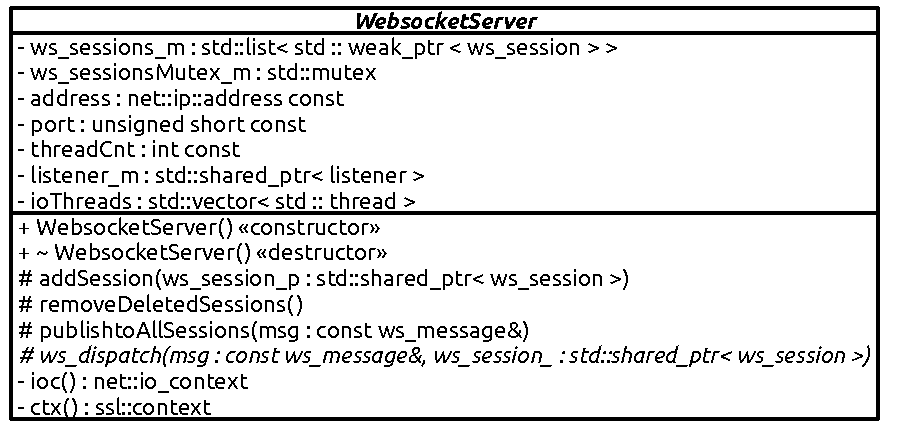
\includegraphics[width=\textwidth]{content/hauptteil/umsetzungPoC/backend/uml/classesOfOverview/WebsocketServer.pdf}
  \caption{Klassendiagramm der Klasse \eigenName{WebsocketServer}}
  \label{fig:backend:classDiag:WebsocketServer}
\end{figure}
Die Klasse \eigenName{WebsocketServer} (\refFig{fig:backend:classDiag:WebsocketServer}) verwaltet die offenen Websocket Sessions (Objekte der Klasse \eigenName{ws\_session}).
Sie bedient sich dabei der bekannten  C++ Bibliothek \eigenName{Boost.Beast} \citep{beast:lib}.
Websocket Sessions sind die einzelnen Verbindungen zwischen Backend und Frontend.
Das Aufbauen von Verbindungen ist den Beispielen von Vinnie Falco zur \eigenName{Boost.Beast} Bibliothek entnommen \citep{beast:examples}.
Die \eigenName{WebsocketServer} Klasse speichert dabei, pro aktiver Websocket Session, einen Pointer des zugehörigen \eigenName{ws\_session} Objekts in einer Liste.
Diese Liste existiert als das Attribut \eigenName{ws\_sessions\_m} in der Klasse \eigenName{WebsocketServer} und ist zusätzlich durch ein Mutex geschützt.
Diese Mutex kann man sich vorstellen wie ein Schloss, das immer zuerst gesperrt werden muss, 
bevor die Session Liste verfügbar ist (Aufruf von \eigenName{std::mutex::lock()}). 
Ist das Mutex von einem Thread gesperrt, so kann ein anderer Thread es solange nicht sperren wie es noch gesperrt ist.
Damit wird der zeitgleiche Zugriff von mehreren Threads auf eine Datenstruktur verhindert (Race Conditions werden verhindert).
Wäre das nicht der Fall könnte es beispielsweise passieren dass ein Element gleichzeitig gelöscht wird, während ein anderer Thread lesend auf das Element zugreift.
Solche Race Conditions bedarfen keiner echten Simultanität (mehrere Prozessorkerne die auf den selben Speicherbereich zugreifen), sie können auch durch das Scheduling des Betriebssystem entstehen. 
Ist ein Thread nun mit der Arbeit an der geschützten Ressource fertig, gibt er sie wieder frei indem er die Methode \eigenName{std::mutex::unlock()} aufruft.
Das scheint der einfachste Weg zu sein, aber nicht der sicherste. 
Wenn im Code zwischen \eigenName{lock()} und \eigenName{unlock()} eine Exception eintritt, 
wird zwar die Ressource danach nichtmehr benötigt, es wird aber auch nicht \eigenName{unlock()} aufgerufen.
Man spricht in diesem Fall von einem \emph{Deadlock}, da das Mutex von einem Thread gesperrt wurde und nie wieder entsperrt wird. 
Das führt dazu, dass alle anderen Threads, die die Ressource benötigen, endlos auf deren Freigabe warten. 
Um das zu verhindern bietet die \ac{stl} eine \eigenName{lock\_guard} Klasse, die bei ihrer Zerstörung das Mutex selbständig wieder frei gibt.
Diese Vorgehensweise sieht man in \refList{list:addSession}, wenn der \eigenName{lock\_guard} in Zeile 354 nicht mehr im Scope ist, wird automatisch \eigenName{unlock()} aufgerufen.
\begin{listing}[ht]
  \inputminted[linenos=true,breaklines=true, firstline=348, lastline=354]{c++}{../Backend/WebsocketServer.cpp}
  \caption{Methode \eigenName{addSession} der Websocket Server Klasse}
  \label{list:addSession}
\end{listing}
\begin{figure}[ht]
  \centering
  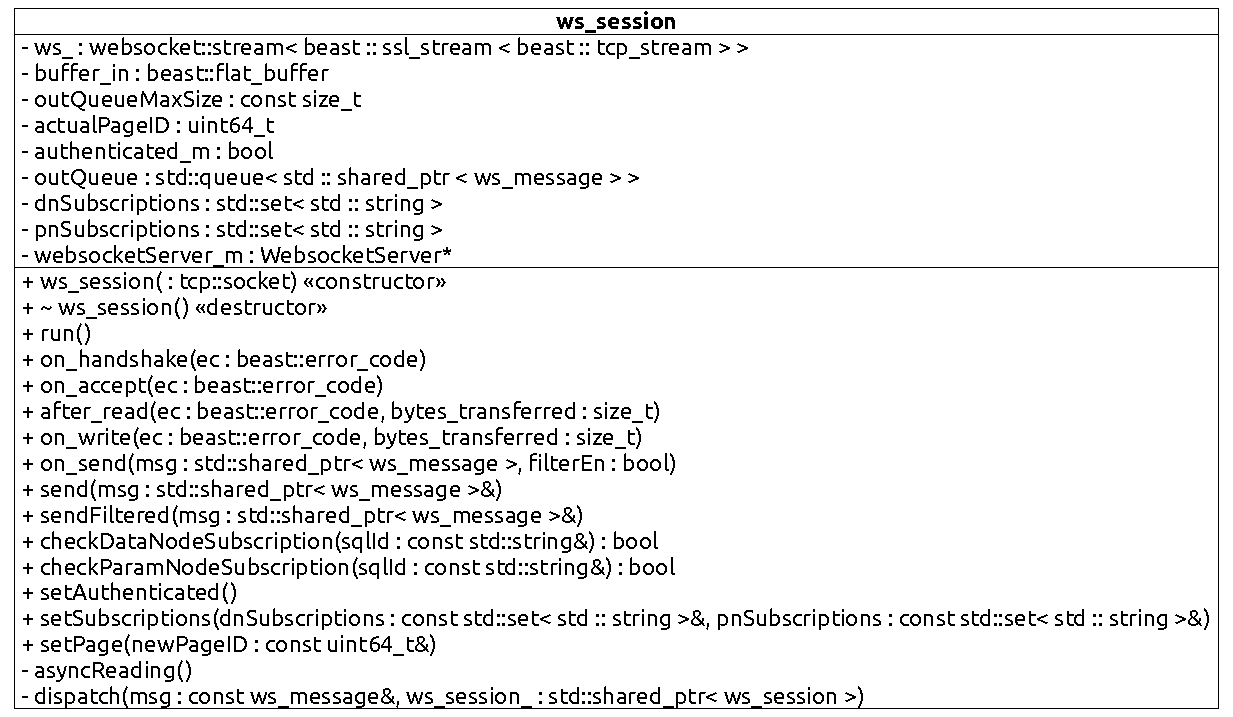
\includegraphics[width=\textwidth]{content/hauptteil/umsetzungPoC/backend/uml/classesOfOverview/ws_session.pdf}
  \caption{Klassendiagramm der Klasse \eigenName{ws\_session}}
  \label{fig:backend:classDiag:wsSession}
\end{figure}
Bei jeder neuen Websocket Verbindung wird ein neues \eigenName{ws\_session} Objekt (Klassendiagramm \refFig{fig:backend:classDiag:wsSession}) instanziert 
und bekommt dabei einen Pointer auf das \eigenName{WebsocketServer} Objekt. Dies ermöglicht dem \eigenName{ws\_session} Objekt 
sich bei dem \eigenName{WebsocketServer} Objekt anzumelden. 
Zusätzlich speichert das \eigenName{ws\_session} Objekt den Pointer unter dem Attribut \eigenName{websocketServer\_m} ab.
Dies ermöglicht es beim Empfang eines kodierten Strings durch das \eigenName{ws\_session} Objekt, ein \eigenName{ws\_message} Objekt aus dem String zu konstruieren
und die virtuelle Methode \eigenName{ws\_dispatch} der \eigenName{WebsocketServer} Klasse aufzurufen, welche in der \eigenName{Backend} Klasse reimplementiert wird.
Dort wird das \eigenName{ws\_message} Objekt dann entsprechend seines Events interpretiert und der entsprechende Handler (beschrieben in Abschnitt \ref{subsec:protokollBackendFrontend}, 
implementiert in der Methode \eigenName{ws\_dispatch}) ausgeführt.
Daten, die in die andere Richtung fließen, werden entweder direkt aus der Dispatcher Methode des Backends in eine einzelne Session geschickt (Aufruf der Methode \eigenName{send} des \eigenName{ws\_session} Objekts), 
oder über die Methode \eigenName{publishToAllSessions} der \eigenName{WebsocketServer} Klasse.
Dabei ist eine Art Publish/Subscribe Mechanismus implementiert, bei dem Änderungen die DataNodes oder ParamNodes betreffen nur dann über die jeweilige Websocket Session an das Frontend gesendet werden, 
wenn eine entsprechende Seite dargestellt ist, welche die Nodes auch verwendet.
\begin{figure}[ht]
  \centering
  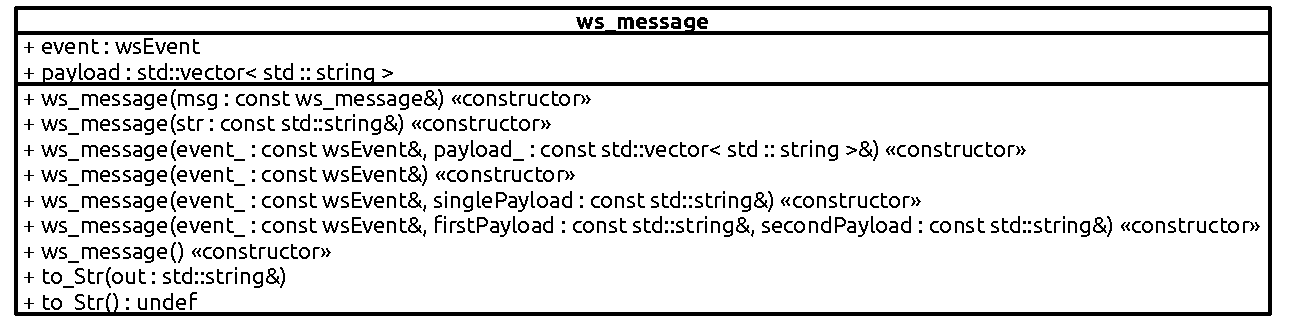
\includegraphics[width=\textwidth]{content/hauptteil/umsetzungPoC/backend/uml/classesOfOverview/ws_message.pdf}
  \caption{Klassendiagramm der Klasse \eigenName{ws\_message}}
  \label{fig:backend:classDiag:wsMsg}
\end{figure}
Bei der Kommunikation mit dem Frontend werden, entsprechend des Abschnitts \ref{subsec:protokollBackendFrontend}, Strings ausgetauscht. 
Diese Strings werden beim Empfang in einem \eigenName{ws\_message} Objekt (Klassendiagramm in \refFig{fig:backend:classDiag:wsMsg}) gespeichert und zum Dispatcher transportiert. 
Dort kann dann auf die einzelnen Komponenten der Nachricht (Event und Payloadvektor) einzeln zugegriffen werden.
Außerdem ermöglicht die Klasse durch die Methode \eigenName{to\_Str} es ihren Inhalt wieder als String, zum Transport an das Frontend, zu kodieren.
Um den Code bei der Verwendung des \eigenName{ws\_message} Objekts so kurz wie möglich zu halten, stehen zum Konstruieren eine Vielzahl von Konstruktoren zur Verfügung.

\subsection{SqlClient}
Die \eigenName{SqlClient} Klasse verwaltet die Verbindung zum \ac{sql} Server. \\Auf dem \ac{sql} Server sind alle Daten gespeichert, die persistiert werden müssen. 
Das Klassendiagramm der \eigenName{SqlClient} Klasse ist in \refFig{fig:backend:classDiag:SqlClient} dargestellt.
Die Klasse bedient sich dabei der offiziellen Bibliothek \eigenName{MariaDB Connector/C API} der OpenSource Datenbank-Engine MariaDB \citep{mariaDB}.
\begin{figure}[ht]
  \centering
  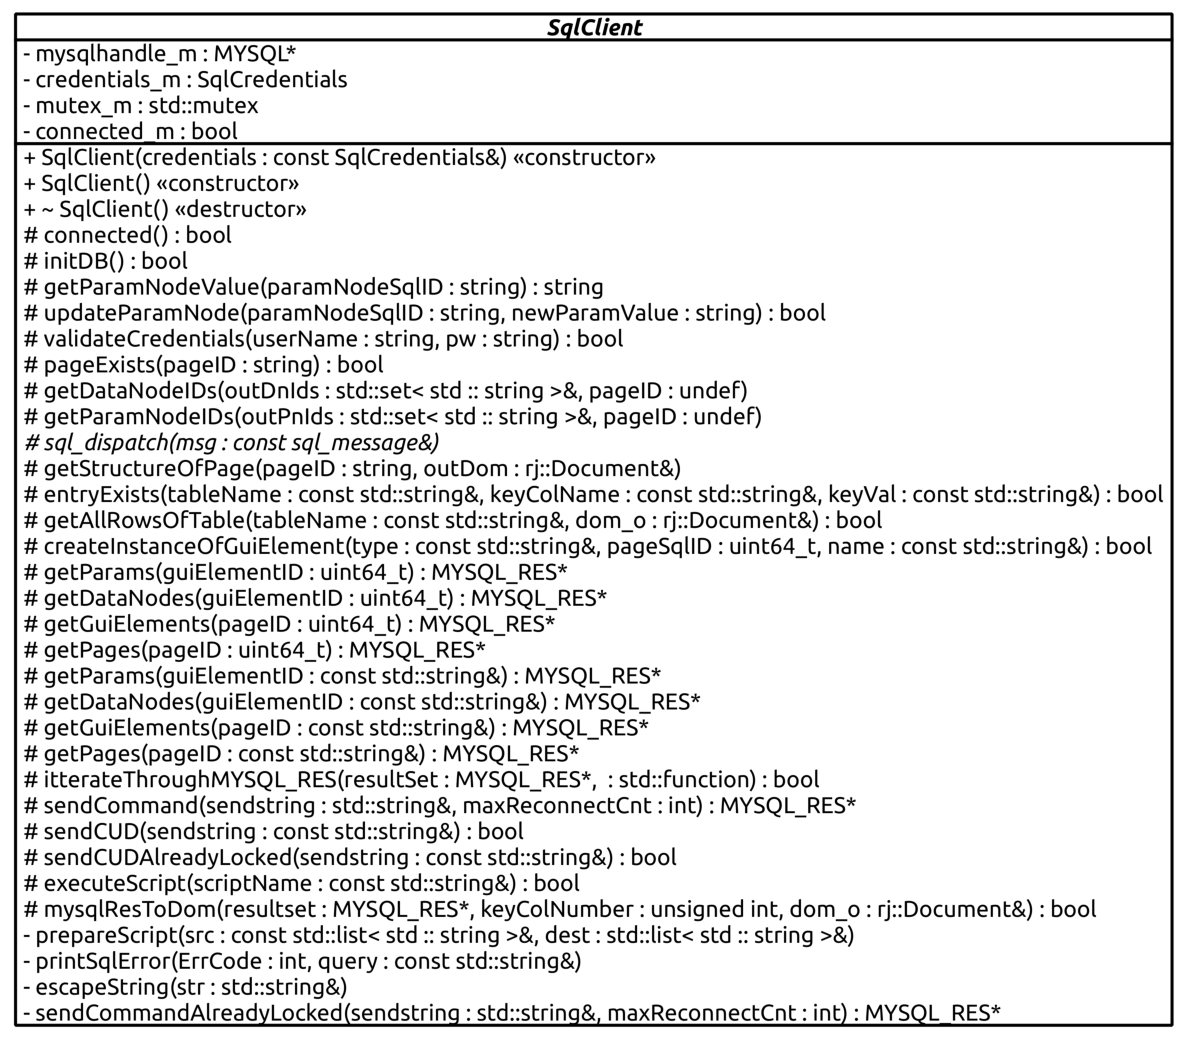
\includegraphics[width=\textwidth]{content/hauptteil/umsetzungPoC/backend/uml/classesOfOverview/SqlClient.pdf}
  \caption{Klassendiagramm der Klasse \eigenName{SqlClient}}
  \label{fig:backend:classDiag:SqlClient}
\end{figure}
Die Datenstruktur des Servers ist in Abschnitt \ref{subsec:dataBackend} beschrieben und dort in \refFig{img:erd} dargestellt.
Diese Struktur ist auf dem \ac{sql} Server vorhanden und wird durch das Skript in \refList{list:createSqlTables} auf dem externe Server konstruiert.
Die \eigenName{SqlClient} Klasse kann mit der Methode \eigenName{executeScript} ein \ac{sql} Skript als Datei ausführen, indem sie es in einzelne Querys zerteilt und diese dann einzeln an den Server sendet.
Das Zerteilen eines Skript und das Vorbereiten zur Ausführung ist in der Methode \eigenName{prepareScript} implementiert. 
Beim Testen der Methode hat sich herausgestellt, dass diese Funktionalität der \eigenName{sql} Client Klasse Skripte auszuführen, schwieriger zu implementieren ist als anfangs vermutet.
Dies liegt daran, dass das Definieren von \emph{stored Procedures} (siehe Abschnitt \ref{subsec:storedProc}) es nötig macht das Semikolon als Trennzeichen zu ändern, 
da in einem Query der Quellcode vorhanden ist, der selbst aus mehreren Querys besteht, die mit einem Semikolon getrennt sind.
Ist ein Skript vorbereitet, so können die einzelnen Querys des Skripts durch den Aufruf der Methode \eigenName{sendCUD} auf dem Server ausgeführt werden.
Die Methode \eigenName{sendCUD} bedient sich dabei der Methode \eigenName{sendCommand}, die die Query an den Server weiterleitet.
Da die Verbindung zum \ac{sql} Server eine geteilte Ressource ist, ist der Zugriff darauf durch \eigenName{sendCommand} durch ein Mutex geschützt, sodass immer nur ein Thread gleichzeitig ein Query senden kann.
Die Klasse \eigenName{SqlClient} bietet viele Methoden um die Daten in der Datenbank abzufragen oder zu verändern.
Um Daten abzufragen werden meistens Querys ausgeführt, die mit \eigenName{Select} beginnen.
Allerdings sind ein paar komplizierte Querys in \emph{stored Procedures} auf dem Server ausgelagert.
Die Prozeduren werden durch das Skript \eigenName{createProcedures} (siehe Anhang \refList{list:createProcedures}) erzeugt.
Um ein \ac{gui} Element zu instanzieren, sind eine Menge an Operationen notwendig.
Diese Operationen sind auch als Prozeduren implementiert und werden durch eine einfache \eigenName{Call} Query aufgerufen.
Immer wenn der Wert einer \emph{ParamNode} auf dem \ac{sql} Server durch Aufruf der Methode \eigenName{updateParamNode} geändert wird, werden alle verbunden \eigenName{ws\_session} Objekte darüber informiert.
Diese Funktionalität ist implementiert, indem in der \eigenName{updateParamNode} Methode zuerst geprüft wird, ob die Änderung tatsächlich eine Änderung darstellt, oder ob der Wert bereits dem neuen Wert entspricht.
Ist das der Fall, wird versucht den Wert auf dem \ac{sql} Server zu ändern. War die Änderung erfolgreich, wird ein \eigenName{sql\_message} Objekt (siehe Klassendiagramm in \refFig{fig:backend:classDiag:sqlMsg}) erstellt 
und der Methode \eigenName{sql\_dispatch} der Klasse \eigenName{SqlClient} übergeben. 
\begin{figure}[ht]
  \centering
  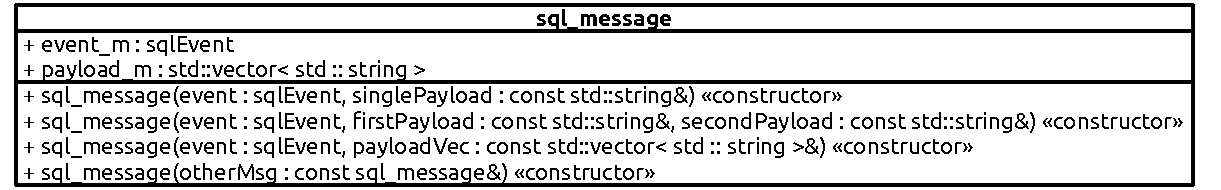
\includegraphics[width=\textwidth]{content/hauptteil/umsetzungPoC/backend/uml/classesOfOverview/sql_message.pdf}
  \caption{Klassendiagramm der Klasse \eigenName{sql\_message}}
  \label{fig:backend:classDiag:sqlMsg}
\end{figure}
Die Datenstruktur des \eigenName{sql\_message} Objekts ist dabei ähnlich aufgebaut wie die des \eigenName{ws\_message} Objekts.
Es besitzt ein Event und ein Payloadvektor.
Die Methode \eigenName{sql\_dispatch} ist in der Klasse \eigenName{Backend} reimplementiert und reagiert auf das \eigenName{sql\_message} Objekt je nach Event.
In diesem Fall ist das Event \eigenName{paramNodeChange}. Hier wird der Payloadvektor so interpretiert, dass das erste Element die NodeID ist und das zweite der neue Wert.
Diese Information wird dann schließlich als \eigenName{ws\_message} kodiert und die Methode \eigenName{publishToAllSessions} der \eigenName{WebsocketServer} Klasse aufgerufen, 
welche diese Information dann an alle Sessions weiterleitet.
In jeder Methode, in der Daten der Websocket Schnittstelle in Querys verwendet werden, können diese nicht als \glqq \mintinline{c++}{const std::String}\grqq{} übergeben werden, da diese durch die Methode \eigenName{escapeString} verändert werden um eine \emph{SQL-Injection} vorzubeugen.
Diese Methode bedient sich dazu einer entsprechenden Funktion der verwendeten Bibliothek.
Würde der String als \glqq \mintinline{c++}{const}\grqq{}  übergeben werden, könnte die Methode den String nicht verändern.

%kurze Erwähnung sinn der klasse
%datenaustausch zwischen SqlClient zu abgeleitetrer...(dispatcher.... ) (I/O)

%beschreibung msg klasse mit diagram

%dispatcher codeausschnitt
%beschreibung dispatcher
\subsection{OpcuaServer}
Die Klasse \eigenName{OpcuaServer} (\refFig{fig:backend:classDiag:OpcuaServer}) implementiert einen \ac{opcua} Server, um die \emph{DataNodes} des \ac{scada} Systems einer Menge an \acp{plc} zugänglich zu machen.
Sie bedient sich dabei der C Bibliothek \eigenName{open62541} \citep{open62541:lib}.
Der Entscheidung für diese Bibliothek liegt die sehr gute Dokumentation der Bibliothek zugrunde.
\begin{figure}[ht]
  \centering
  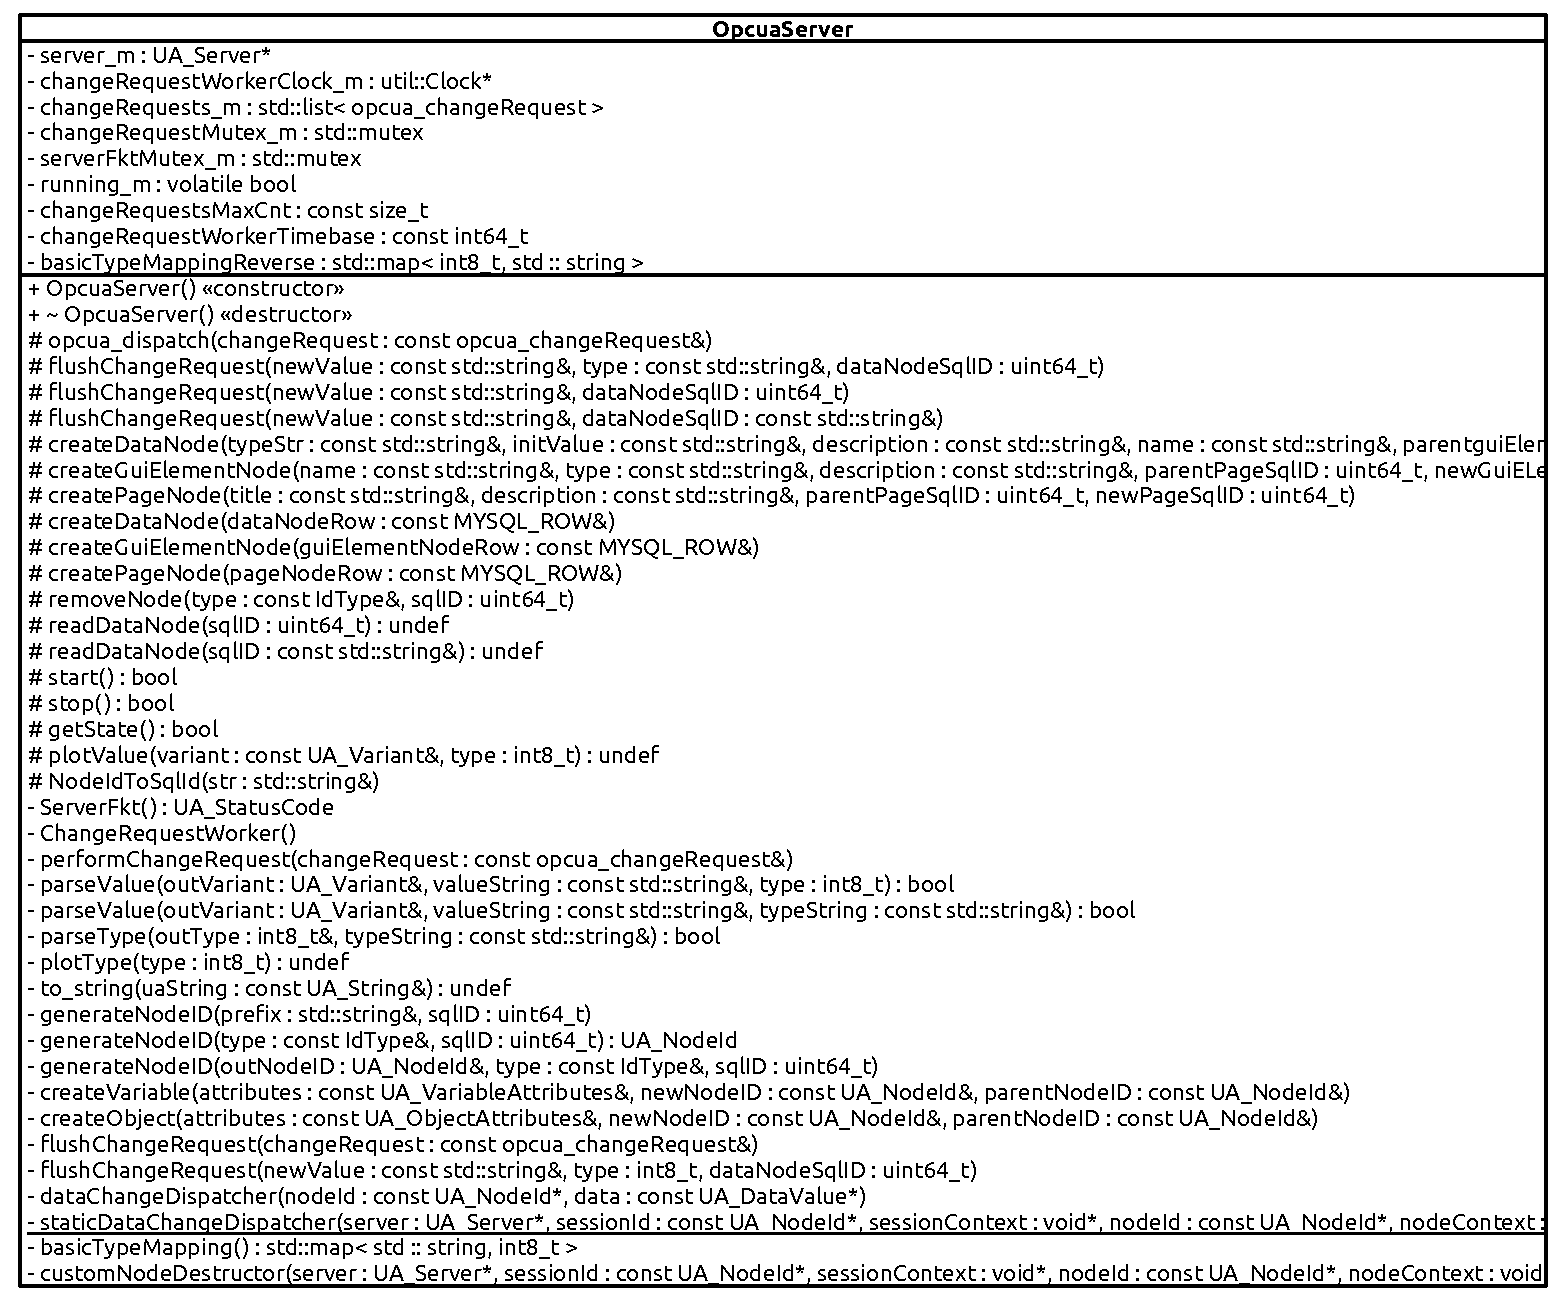
\includegraphics[width=\textwidth]{content/hauptteil/umsetzungPoC/backend/uml/classesOfOverview/OpcuaServer.pdf}
  \caption{Klassediagramm der Klasse \eigenName{OpcuaServer}}
  \label{fig:backend:classDiag:OpcuaServer}
\end{figure}
Das Datenmodell des \ac{opcua} Servers beinhaltet nur die eigebauten Datentypen, also nur primitive Typen (Bool, String, Int \dots) und den Typ \emph{Object}.
auf die Erstellung eines Datenmodells für jeden \emph{GuiElement} Typ wurde verzichtet, da diese an dieser Stelle nur zur Strukturierung der \emph{DataNodes} verwendet werden.
Die Datenstruktur die den \acp{plc} zur Verfügung gestellt wird, einhält eine \emph{Page} die wiederum eine \emph{Page} enthalten kann oder ein oder mehrere \emph{GuiElements}
Jedes \emph{GuiElement} hat DataNodes deren Typ, entsprechend der Vorlage des \emph{GuiElement} Typs in der \ac{sql} Datenbank festgelegt ist.
Die Übersetzung der Typen ist dabei durch das Attribut \eigenName{basicTypeMapping} definiert, das die in der Datenbank gespeicherten Typ Strings auf die eingebauten \ac{opcua} Datentyp mappt.
Die Umkehrung des Mappings ist in dem Attribut \eigenName{basicTypeMappingReverse} gespeichert.
Die Klasse \eigenName{OpcuaServer} stellt den anderen Klasses des Backends Methoden zur Verfügung um \emph{DataNodes}, \emph{GuiElements} und \emph{Pages} auf dem OpcuaServer zu erstellen.
Die Methode \eigenName{readDataNode} ermöglich das Auslesen einer einzelnen \emph{DataNode}. Sie wird verwendet wenn eine Seite im Frontend neu geladen wird und noch keine Daten vorhanden sind.
Daten können entweder über die \ac{opcua} Schnittstelle geändert werden, oder durch eine Anforderung des Backends selbst.
Muss der Wert einer \emph{DataNode} geändert werden, so muss ein \eigenName{opcua\_changeRequest} Objekt erstellt werden (siehe Klassendiagramm in \refFig{fig:backend:classDiag:opcuaCR}), 
das die \eigenName{nodeID} und den neuen Wert der DataNode beinhaltet. Dieses Objekt wird anschließend an die Methode \eigenName{flushChangeRequest} übergeben.
\begin{figure}[ht]
  \centering
  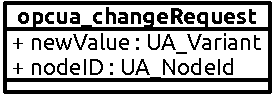
\includegraphics[width=0.2\textwidth]{content/hauptteil/umsetzungPoC/backend/uml/classesOfOverview/opcua_changeRequest.pdf}
  \caption{Klassediagramm der Klasse \eigenName{opcua\_changeRequest}}
  \label{fig:backend:classDiag:opcuaCR}
\end{figure}
Das \eigenName{OpcuaServer} Objekt hat drei Threads. Ein Thread der exclusiv dem nativen Server der \emph{opne62541} Bibliothek zugeordnet ist und zwei Threads mit denen zyklisch geprüft wird, 
ob \eigenName{opcua\_changeRequest} Objekte in der Warteschlange (Attribut \eigenName{changeRequests\_m}) vorhanden sind.
Sind in der Warteschlange \eigenName{opcua\_changeRequest} Objekte vorhanden, wird jedes Element an die Methode \eigenName{performChangeRequest} übergeben und aus der Warteschlange entfernt.
In der Methode \eigenName{performChangeRequest} wird dann die Änderung an der Datenstruktur durchgeführt.% eventuell noch den Trick mit NodeContext erklären () void*.....
Bei der Erstellung jeder \emph{DataNode} wird ein Handler angemeldet, der bei jedem Schreibvorgang auf die Node aufgerufen wird.
Dieser Handler ist als die Methode \eigenName{dataChangeDIspatcher} implementiert.
In diesem Handler wird verglichen, ob der Schreibvorgang ein Änderung des Werts darstellt. Ist das der Fall, wird die Methode \eigenName{opcua\_dispatch} mit einem \eigenName{opcua\_changeRequest} aufgerufen, der die nodeID sowie den neuen Wert Der \emph{DataNode} enthält.
Diese Methode wird schließlich in der \eigenName{Backend} Klasse reimplementiert und leitet die Änderung an die \eigenName{WebsocketServer} Klasse weiter. 